\chapter{Desarrollo del trabajo}  
%\addcontentsline{toc}{chapter}{\numberline{}Desarrollo del trabajo}

\section{Arquitectura y diseño de base de datos}

\subsection{Base de datos}

A continuación, se expone el diseño de la base de datos de cada perfil de usuario.

\begin{itemize}
	\item \texttt{configuration}: Es la única entidad sin relaciones con otras tablas. Tiene dos elementos, \texttt{key} y \texttt{value}. \todo
	\item \texttt{language}: Contiene información sobre los idiomas que el usuario está estudiando. Tiene los siguientes atributos:
		\begin{itemize}[label=$\star$]
			\item \texttt{id}: Identificador único del idioma.
			\item \texttt{name}: Nombre del idioma.
			\item \texttt{dictionary\_url}: URL al diccionario \textit{online} que se incrusta debajo del formulario de edición de los datos de palabras.
			\item \texttt{should\_show\_spaces}: Si tiene valor $1$, los espacios que contenga un texto se renderizarán con normalidad; en cambio, si tiene valor $0$, los espacios serán invisibles. Esto resulta útil en el caso de idiomas que no suelen separar las palabras mediante espacio, como el japonés o los idiomas chinos, para que, aunque la aplicación requiera algún carácter entre las distintas palabras para su correcto funcionamiento, esto no afecte negativamente a la experiencia del usuario.
			\item \texttt{alphabet}: Expresión regular que describe los caracteres que conforman las palabras del idioma.
			\item \texttt{sentence\_delimiters}: Expresión regular que describe los caracteres que denotan el final de un enunciado en el idioma.
			\item \texttt{whitespaces}: Expresión regular que describe los caracteres que denotan la separación entre palabras.
			\item \texttt{intraword\_punctuation}: Expresión regular que describe los caracteres que, aun no siendo parte del alfabeto, pueden aparecer en medio de una palabra.
			\item \texttt{template\_code}: Identificador de la plantilla utilizada como base para configurar el idioma.
			\item \texttt{script\_name}: \todo
			\item \texttt{text\_processors}: Lista de procesadores de texto que se ejecutan al importar textos en este idioma.
			\item \texttt{word\_data\_provider}: Proveedor de datos de palabras que se utilizará para autocompletar el formulario de modificación de palabra cuando se consulte una nueva palabra en este idioma.
		\end{itemize}
	\item \texttt{word}: Contiene información acerca de las palabras alguna vez vistas por el usuario. Contiene los siguientes atributos:
	\begin{itemize}[label=$\star$]
		\item \texttt{id}: Identificador único de la palabra.
		\item \texttt{language\_id}: Identificador del idioma al que pertenece la palabra.
		\item \texttt{content}: Secuencia de caracteres que conforman la palabra.
		\item \texttt{status}: Nivel de familiarización del usuario con la palabra. Vale $1$ para palabras que el usuario solo haya visto una vez, y aumenta gradualmente hasta $5$ para palabras que sean prácticamente del todo familiares para el usuario. Una vez el usuario marque la palabra como aprendida, el valor de \texttt{status} será $99$. Se reserva el valor $98$ para palabras que deben ser ignoradas: según la metodología del estudiante, puede usarse para nombres propios, para palabras inexistentes (que pueden emerger con motivo del funcionamiento imperfecto de los analizadores sintácticos) o para palabras que no pertenecen al idioma en cuestión.
		\item \texttt{notes}: Anotaciones sobre la palabra.
		\item \texttt{time\_added}: \textit{Timestamp} del momento de creación de la palabra.
		\item \texttt{time\_updated}: \textit{Timestamp} del momento de última actualización de la palabra.
		\item \texttt{token\_count}: Número de \textit{tokens} que conforman la palabra. Es útil para formas complejas como locuciones, que están formadas por varias palabras pero actúan para muchos efectos como una sola.
	\end{itemize}
	\item \texttt{entry}: Entrada de diccionario de una palabra.
	\begin{itemize}[label=$\star$]
		\item \texttt{id}: Identificador único de la entrada.
		\item \texttt{word\_id}: Identificador de la palabra a la que corresponde la entrada.
		\item \texttt{position}: Posición en la que se coloca la entrada.
		\item \texttt{meaning}: Acepciones de la palabra según esta entrada.
		\item \texttt{reading}: Lectura de la palabra según esta entrada.
	\end{itemize}
	\item \texttt{word\_status\_log}: Histórico de cambios realizados al estado de las palabra.
	\begin{itemize}[label=$\star$]
		\item \texttt{id}: Identificador único del cambio.
		\item \texttt{word\_id}: Identificador de la palabra a la que corresponde el cambio.
		\item \texttt{status}: Nuevo estado de la palabra.
		\item \texttt{time\_updated}: \textit{Timestamp} del momento en que se realizó el cambio.
	\end{itemize}
	\item \texttt{text}: Contiene información acerca de un texto.
	\begin{itemize}[label=$\star$]
		\item \texttt{id}: Identificador único del texto.
		\item \texttt{language\_id}: Identificador del idioma en que está escrito el texto.
		\item \texttt{title}: Título del texto.
		\item \texttt{source\_url}: URL de la página web de la que se importó el texto, en caso de que aplique.
		\item \texttt{time\_opened}: \textit{Timestamp} del momento en que se abrió el texto por última vez.
		\item \texttt{time\_finished}: \textit{Timestamp} del momento en que se terminó de leer el texto por completo.
		\item \texttt{progress}: Valor entre $0$ y $1$ que indica el porcentaje de páginas del texto que el usuario ha leído.
	\end{itemize}
	\item \texttt{page}: Página de un texto.
	\begin{itemize}[label=$\star$]
		\item \texttt{id}: Identificador único de la página.
		\item \texttt{text\_id}: Identificador del texto al que pertenece la página.
		\item \texttt{position}: Posición en la que se coloca la página.
		\item \texttt{content}: Contenido de la página.
	\end{itemize}
	\item \texttt{text\_progress\_log}: Histórico de cambios realizados al progreso de un texto.
	\begin{itemize}[label=$\star$]
		\item \texttt{id}: Identificador único del cambio.
		\item \texttt{text\_id}: Identificador del texto al que corresponde el cambio.
		\item \texttt{progress}: Nuevo progreso de la palabra.
		\item \texttt{time\_updated}: \textit{Timestamp} del momento en que se realizó el cambio.
	\end{itemize}
\end{itemize}

\begin{figure}
	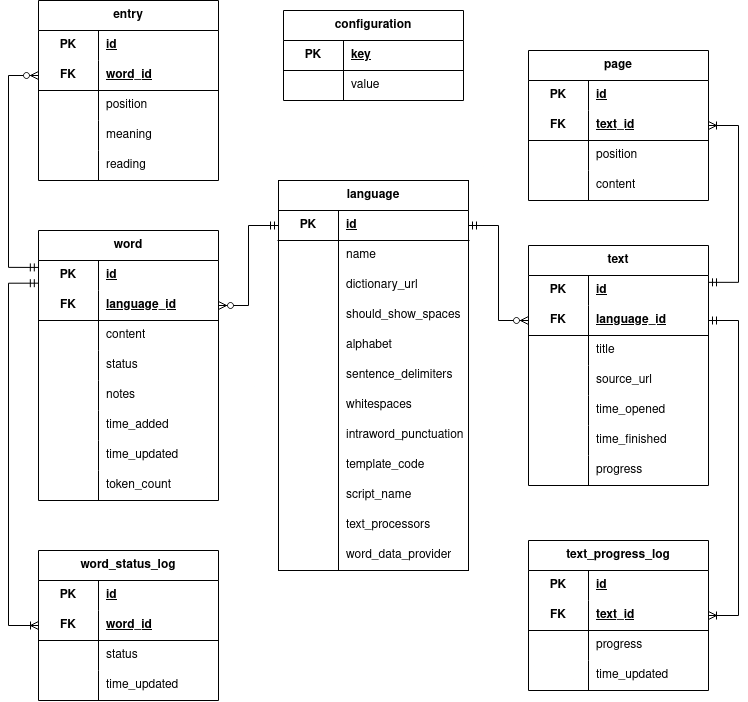
\includegraphics[width=1\textwidth]{er-diagram.drawio.png}
	\caption[Diagrama entidad-relación]{Diagrama entidad-relación con notación \textit{Crow's foot}.}
\end{figure}

Diagrama frontend vs backend, incluir plugins, incluir sistema de archivos.

Todo con explicación, evidentemente.
	
\section{Implementación de necesidades lingüísticas}

Relacionar historias de usuario con trozos del código, haciendo referencias a las hipótesis de Krashen.

\section{Diseño UI/UX}

Explicar diseño. Leyes Gestalt, teoría de colores y esas cosas. Diseño responsive también. Accesibilidad.

\section{Proceso de desarrollo}

Agile llevado a la práctica.

Decir algo sobre \textit{feedback}.
